\documentclass[12pt]{article}
\usepackage[margin=0.8in]{geometry}
\usepackage{physics}
\usepackage{graphicx}
\usepackage{amsmath}

\begin{document}
\title{User Guide for Reduced-Hamiltonian Taylor Coefficient Generation}
\author{Jake Smith \\ jsmith74@tulane.edu}
\maketitle

\tableofcontents
\section{Compiling the C++ Code}
Before we begin, we need to compile some C++ code. A makefile is included with the source files, that will automatically build a binary executable and call it \textit{RTCGen}. Some non-standard libraries are required:
\begin{itemize}
\item libuuid
\item Eigen3 
\item WSTP 
\end{itemize}
Eigen3 and WSTP should be included with the source code files pulled from the TeamForge git repository, and require no additional installation. If you want to compile this program on an OS other than Linux, you will need to replace the WSTP library with the version included with your installation of \textit{Mathematica.} Uuid is available through standard package repositories- yum on CentOS, or apt-get on Ubuntu. 
\newline
\newline
The user should never need to recompile any code; \textit{RTCGen} was written to be completely general. All physical and algorithm control parameters are input via a \textit{Mathematica} notebook.
\section{Running the Code and Reading the Output}
\subsection{A Quick How-to-Use Guide}
This purpose of this program is to approximate a large user-defined Hamiltonian in some small dimensional Hilbert space, and to Taylor expand this result. This will allow an efficiently repeatable after-the-fact consideration of noise in a physical simulation.
\newline
\newline
For the purpose of usability, the \textit{RTCGen} was written to allow the user to input all physical definitions in a \textit{Mathematica} notebook. These definitions are:
\newline
\newline
\begin{itemize}
\item The eigen decomposition of a "large" Hamiltonian in some initial basis as a function of a set of flux parameters
\newline
\item A predefined, time-dependent ideal (free of noise) path through flux space
\newline
\newline
\end{itemize}

In order to define the eigen decomposition of the Hamiltonian, we write a function in \textit{Mathematica} called \textbf{es}, which takes in a vector position in flux space and returns a (possibly truncated) list of eigenvalues and eigenvectors of our full Hamiltonian. E.g. for the prototypical two level system with flux parameters $\varepsilon$ and $\Delta$,
\begin{equation}
 H(\varepsilon(t),\Delta(t)) = \frac{1}{2}\begin{bmatrix}
    \varepsilon(t) & \Delta(t)  \\
    \Delta(t) & -\varepsilon(t) 
  \end{bmatrix}
\end{equation}
we can write the \textit{Mathematica} function
\begin{equation}
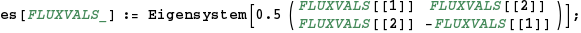
\includegraphics[scale=0.75]{es.png}
\end{equation}
The output of \textbf{es} must be a \textit{Mathematica} List of two elements; the first being a List of eigenvalues, and the second being a List of corresponding eigenvectors. The eigensystem must be order in order of increasing eigenvalues, and all eigenvectors must be normalized. This is usually the format of the output of \textit{Mathematica}'s built in eigen-solver, \textbf{Eigensystem}, and  is the format of the realistic flux qubit eigen-decomposition Jamie provided. Occasionally, \textbf{Eigensystem} will not output in this format by default - the eigenvalues will not be ordered or the eigenvectors will not be normalized. You may need to add some extra code to fix this.
\newline
\newline
In order to define the ideal path through flux space, we write a function \textbf{fluxVec}, which takes in a time and returns a vector of instantaneous flux values. E.g. for our Hamiltonian above, say we want to follow the ideal flux path:
\begin{equation}
\varepsilon(t) = \frac{1}{4} \cos(2.0 \pi t) \quad \Delta(t) = 11.0
\end{equation}
then we write a \textit{Mathematica} function,
\begin{equation}
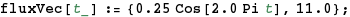
\includegraphics[scale=0.75]{fv.png}
\end{equation}
The output of \textbf{fluxVec} must be a List of Real numbers representing a position in flux space.
\newline
\newline
Next, the user can choose the output file directory; the location where the Taylor coefficients and any debugging files will be saved by using the standard \textbf{SetDirectory} function:
\begin{equation}
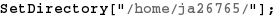
\includegraphics[scale=0.75]{sd.png}
\end{equation}
Now, we need to link our notebook to the compiled Taylor coefficient generator program. This is done with \textit{Mathematica}'s \textbf{Install} function. By default, I've named our compiled program \textit{RTCGen} in the makefile, so the proper function call would be (assuming the binary was in my home directory)
\begin{equation}
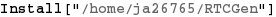
\includegraphics[scale=0.75]{i.png}
\end{equation}
Finally, the user needs to tell \textit{Mathematica} to generate the taylor coefficients of the reduced-Hamiltonian. This is done by calling the function \textbf{GenerateTaylorCoefficients}, with the following arguments:
\begin{equation*}
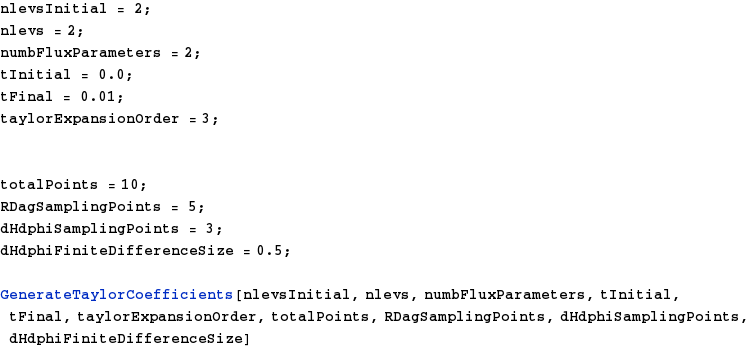
\includegraphics[scale=0.6]{gtc.png}
\end{equation*}
A quick rundown of these arguments:
\begin{itemize}
\item \textbf{nlevsInitial} is the Hilbert space dimension of the large Hamiltonian in the initial energy eigenbasis.
\item \textbf{nlevs} is the reduced Hilbert space dimension of our truncated system
\item \textbf{numbFluxParameters} is the dimension of the flux space
\item \textbf{tInitial} is the starting time for our journey through flux space
\item \textbf{tFinal} is the ending time for our journey through flux space
\item \textbf{taylorExpansionOrder} is the highest order set of coefficients in the taylor expansion that we want the program to evaluate
\newline
\newline
\end{itemize}
The remaining four arguments; \textbf{totalPoints, RDagSamplingPoints, dHdphiSamplingPoints} and \textbf{dHdphiFiniteDifferenceSize} are non-physical parameters that we will go into more detail in section 3.
\newline
\newline 
For now, you should be able to at least \textit{run} this code for any physical system you choose. If successful, running the function \textbf{GenerateTaylorCoefficients} should return the following message:
\begin{equation}
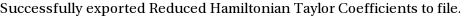
\includegraphics[scale=0.6]{serhtctf.png}
\end{equation}
and the files "\textit{RTC.dat}", "\textit{evH0.dat}", "\textit{Taylor\_Coefficient\_Order.dat}" and "\textit{finalEb.dat}" should appear in the directory specified.
If this message does not appear, and the output files containing the taylor coefficients are nowhere to be found, the reason is likely due to \textit{Mathematica}'s way of implicitly defining variable types; see section 2.2.
\newline
\newline
As a final step, you can unlink my program from your \textit{Mathematica} notebook if you want.
\begin{equation}
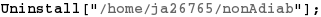
\includegraphics[scale=0.75]{ui.png}
\end{equation}
Neat.
\newline
\newline
Included with the source files and this PDF is an example notebook, \textit{Example Mathematica Notebook.nb} which defines \textbf{es} for the more complicated, realistic flux qubit provided by Jamie, and an arbitrarily chosen pulse signal for \textbf{fluxVec}. 
\subsection{Data Types}
\begin{figure} [h!]
\begin{center}
    \begin{tabular}{  l| l  }

    nlevsInitial & Integer  \\ 
    nlevs & Integer  \\ 
    numbFluxParameters & Integer \\ 
    tInitial & Real  \\ 
    tFinal & Real  \\ 
    taylorExpansionOrder & Integer  \\ 
    totalPoints & Integer  \\ 
    RDagSamplingPoints & Integer (must be odd)  \\ 
    dHdphiSamplingPoints & Integer (must be odd)  \\ 
    dHdtFiniteDifferenceSize & Real
    \end{tabular}
\end{center}
\caption{Parameters and Their Implicitly defined Datatypes}
\label{parameterTable}
\end{figure}
Because we're exchanging data between a compiled C++ binary and a \textit{Mathematica} notebook, the user needs to be at least a little bit aware of how data types are declared in both languages. 
\newline
\newline 
In C++, all variables must be declared with an explicit type (e.g. int, double, long, char, etc).
\newline
\newline
In \textit{Mathematica} all data types are declared implicitly. There are only two numeric types; \textbf{Integer} and \textbf{Real}, which are analogous to C++'s \textbf{int} and \textbf{double}, respectively. The type is assigned depending on if the user included a decimal point in their definition or not:
\newline
\newline
\begin{minipage}[t]{0.5\textwidth}
\centering \textit{C++}
\newline
\newline
\textbf{int} x = 5;
\newline
\textbf{double} x = 5.0;
\newline
\newline
\end{minipage}
\begin{minipage}[t]{0.5\textwidth}
\centering \textit{Mathematica}
\newline
\newline
x = 5;  
\newline
x = 5.0;
\newline
\newline
\end{minipage}
%\newline
%\newline
%\textit{Mathematica} stores complex numbers and arrays (or any other numeric data structure) in \textit{expressions} of \textbf{Integer} and \textbf{Real} data:
%\newline
%\newline
%\begin{minipage}[t]{0.5\textwidth}
%\centering \textit{C++}
%\newline
%\newline
%\textbf{std::complex$<$double$>$} x(3.1,4.5);
%\newline
%\newline
%\textbf{int} x[4];
%\newline
%x[0] = 1; x[1] = 6; x[2] = -3; x[3] = 2;
%\newline
%\newline
%\end{minipage}
%\begin{minipage}[t]{0.5\textwidth}
%\centering \textit{Mathematica}
%\newline
%\newline
%x = Complex[3.1,4.5];
%\newline
%\newline
%x = List[1,6,-3,2];
%\newline
%\newline
%\end{minipage}
%We can check to see how an expression is explicitly being stored in \textit{Mathematica} by using the built-in function \textbf{FullForm};
%\begin{equation}
%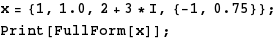
\includegraphics[scale=0.75]{ff.png}
%\end{equation}
%\begin{equation*}
%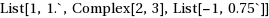
\includegraphics[scale=0.75]{ffr.png}
%\end{equation*}
%Note that a List, unlike an array in C++, can be composed of different data types.
%\newline
%\newline

Calling \mbox{\textbf{GenerateTaylorCoefficients}} in a \textit{Mathematica} notebook will not work unless all of the input parameters are of the correct data type, \textbf{Integer} or \textbf{Real}. For a list of the explicit type definitions, refer to Fig.~(\ref{parameterTable}).
\subsection{Format of the Output}
Running the code successfully will create four data files in the directory specified by the user. These files are
\begin{itemize}
\item \textit{evH0.dat}
\item \textit{RTC.dat}
\item \textit{Taylor\_Coefficient\_Order.dat}
\item \textit{finalEb.dat}
\end{itemize}
 \textit{evH0.dat} contains a series of columns separated by a tabulator character. The first column contains a list of time values; these are the points in time at which you are diagonalizing your "large" Hamiltonian. The remaining columns will be the  \textbf{nlevs} lowest eigenvalues at each time (at least the lowest at \textbf{tInit} - the code should correct any degenerate crossing). \textit{evH0.dat} is generated as a way for the user to verify that everything went alright - plot these values and make sure any crossings went well, and that the resolution is appropriate, if you so desire.
 \newline
 \newline
 \textit{RTC.dat} contains the coefficients for the taylor expansion of our reduced Hamiltonian. This file should be readable to humans in the current version of the code. First, a double precision number gives the starting time \textbf{tInit}. Then , there should be a set of (\textbf{nlevs} by \textbf{nlevs}) complex matrices. These are the taylor expansion coefficients. Then, some extra line breaks, and then the succeeding time value and its corresponding taylor coefficients. This cycle continues over the duration of the time interval specified by the user in the \textit{Mathematica} code. I'll give a short description of what these matrices are in the next section, and then how to use them in the section after that. The format of how these matrices are exported was an arbitrary decision. If you want to change the I/O style, you can edit the commented function at the top of the file \textit{reducedTaylorCofficientGen.cpp}, or send me an email and I'd be happy to change it.
\subsection{Multivariable Taylor Expansion}

The main idea here is that we're expanding our flux-dependent "small" Hamiltonian in the instantaneous eigenbasis around ideal points in flux space, to allow noise-perturbations to be considered later. Formally, lets define

\center{ $\vec{\phi}(t) = \{\phi_1(t),\phi_2(t)...\phi_m(t)\}$}
 as an ideal (noiseless) position in $m$-dimensional flux space at time $t$. This vector is determined by our \textit{Mathematica} function, \textbf{fluxVec}.
\center{$\vec{x}(t) = \{x_1(t),x_2(t)...x_m(t)\}$ as some perturbative vector that represents our flux noise at time $t$. This "noise position" will be incorporated later, during an actual simulation.} 

\flushleft With noise, our position in flux space is therefore $\vec{\phi}(t) + \vec{x}(t)$, and our exact Hamiltonian in the instantaneous eigenbasis at time $t$ is determined by
\begin{equation}
H(\vec{\phi}(t) + \vec{x}(t))
\end{equation}
We parametrize the length of the noise vector and apply taylor's theorem:
\begin{equation}
G(q) = H(\vec{\phi}(t) + q \vec{x}(t))
\end{equation}
\begin{equation}
H(\vec{\phi}(t) + \vec{x}(t)) = G(1) = G(0) + G'(q)|_{q=0} + \frac{1}{2} G''(q)|_{q=0}+...
\end{equation}
Applying the chain rule, we find
\begin{equation}
H(\vec{\phi}(t) + \vec{x}(t)) = \sum_{n=0} \frac{F_n(\vec{x}(t))}{n!}
\end{equation}
where
\begin{equation}
F_n(\vec{x}(t)) = \sum_{r_1,r_2,...,r_n=1}^m \frac{\partial^n H(\vec{\phi}(t)+ \vec{\xi}(t))} {\partial \xi_{r_1}\partial \xi_{r_2}...\partial \xi_{r_n}}  |_{\vec{\xi}=\vec{0}} \quad \cdot  x_{r_1}(t) \cdot x_{r_2}(t) \cdot ... \cdot x_{r_n}(t)
\end{equation}
When running an actual physical simulation, the user must define some time dependent flux-noise function, $x(t)$, and evolve the system with the Hamiltonian,
\begin{equation}
H_{noise}(\vec{x}(t)) = \sum_{n=0}^{N} \frac{F_n(\vec{x}(t))}{n!}
\end{equation}
over each discrete time interval, where $N$ is the expansion order specified by the user.
\newline
\newline
\textbf{The matrices contained in the file \textit{RTC.dat} are the coefficients}
\newline
\begin{equation}
\boxed{C_t(n,\vec{r}) = \frac{\partial^n H(\vec{\phi}(t)+ \vec{\xi}(t))} {\partial \xi_{r_1}\partial \xi_{r_2}...\partial \xi_{r_n}}  |_{\vec{\xi}=\vec{0}}}
\end{equation}
\newline
\textbf{which we have indexed with a vector labeling $\vec{r}$ and expansion order $n$. Thus, the instantaneous Hamiltonian at time $t$, as a function of flux noise is}
\newline
\begin{equation}
\boxed{H_{noise}(\vec{x}(t)) = \sum_{n,\vec{r}} \frac{C_t(n,\vec{r})}{n!} \cdot x_{r_1}(t) \cdot x_{r_2}(t) \cdot ... \cdot x_{r_n}(t)} 
\end{equation}
\newline
\textbf{where $n: 0 \rightarrow N$ and $\vec{r}$ is over all distinct partial derivatives of the $m$ flux variables.}
\newline
\newline
The total number of coefficient matrices, $C_n(t,\vec{r})$ , generated at each point in time depends on the dimension of the flux space, $m$, and the expansion order of our taylor series, $N$:
\begin{equation}
\mbox{Number of } C_t(n,\vec{r}) \mbox{ matrices } =\sum_{n=0}^N \frac{(n+m-1)!}{n!(m-1)!}
\label{numbCoeff}
\end{equation}
Deriving eq.~(\ref{numbCoeff}) is a neat little exercise.
\newline
\newline
The $C_t(n,\vec{r})$ at each time $t$ are printed in \textit{RTC.dat} in a hierarchical order. At the highest priority, the coefficients are in order of taylor expansion order, $n$. Below that, we use reverse lexicographic ordering of the $\vec{r}$ vectors. We can flatten this total ordering into a single index, which I'll just call $l.$ As an example, refer to Fig.~(\ref{coeffOrdering}) the ordering for a system in 2-dimensional flux space expanded to 3rd order.
\begin{figure}[h!]
\begin{center}
    \begin{tabular}{ l l l }
 	$l$ & n & $\vec{r}$ \\ \hline
 	1 & 0 & () \\
 	2 & 1 & (1) \\
 	3 & 1 & (2) \\
 	4 & 2 & (1,1) \\
 	5 & 2 & (1,2) \\
 	6 & 2 & (2,2) \\
 	7 & 3 & (1,1,1) \\
 	8 & 3 & (1,1,2) \\
 	9 & 3 & (1,2,2) \\
 	10 & 3 & (2,2,2)
    \end{tabular}
\end{center}
\caption{Ordering of the $C_t(n,\vec{r})$ Matrices as they are printed in \textit{RTC.dat} for $m=2$ and $N=3$}
\label{coeffOrdering}
\end{figure}
%In my C++ program, all of these coefficient matrices are stored in a single "long" horizontal matrix, organized hierarchically, first by increasing expansion order, and then by reverse lexicographic ordering of the $\vec{r}$ vectors. That sounds way more complicated than it actually is so let's just do an example; say a system in 2-dimensional flux space expanded to 3rd order. Then the taylor coefficients at some time interval $t$ are stored in an (\textbf{nlevs} by $\mbox{\textbf{nlevs}} \cdot \sum_{n=0}^N \frac{(n+m-1)!}{n!(m-1)!}$) dimensional complex matrix, $H_{total}$:
%\begin{figure}[h!]
%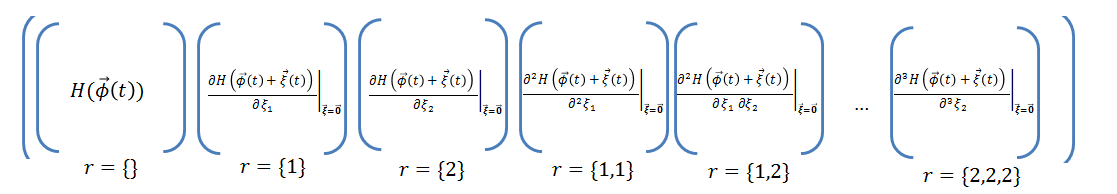
\includegraphics[scale=.58]{Cmat.png}
%\caption{Storage Order of the Taylor Coefficients in a single Large Matrix we'll call $H_{total}$}
%\label{storageOrder}
%\end{figure}
%\newline
%This full matrix is then printed to one line in \textit{H0.dat} in a column major ordering, alternating between real and complex parts of each matrix entry. In other words, the matrix $H_{total}(t)$ will be printed as
%\newline
%$$ \small t \quad \mbox{ "\textbackslash t"} \quad Re(H_{total}(1,1)) \quad \mbox{ "\textbackslash t"} \quad Im(H_{total}(1,1))\quad \mbox{ "\textbackslash t"} \quad Re(H_{total}(2,1)) \quad \mbox{ "\textbackslash t"} \quad Im(H_{total}(2,1)) \quad ... $$
%\newline
%Storing and printing the coefficients this way was somewhat of an arbitrary decision, though Eigen by default stores matrices in a column major ordering, so accessing elements of $H_{total}$ along this path is perhaps a little faster. Still, if you want to change the way the coefficient matrices are written to the disc, you can do so by editing the commented function at the top of \textit{reducedTaylorCoefficientGen.cpp}. Or feel free to email me, and I can change the output to your liking.
\subsection{Direct step-by-step Instructions for using \textit{H0.dat} to build the Hamiltonians with noise in your simulation}
The following are the steps for building the approximation to the Hamiltonian with flux-noise, $H_{noise}(\vec{x}(t))$ at each time, $t$:
\newline
\newline
First, import the complex matrices in the order they are saved in \textit{RTC.dat} and index them in order with a single integer $l$. Call these matrices $C_t(l)$.
\newline
\newline
Open \textit{Taylor\_Coefficient\_Order.dat}. Each line in this file is a vector of integers similar to the $\vec{r}$ vector of the previous section. There should be $\sum_{n=0}^N \frac{(n+m-1)!}{n!(m-1)!}$ vectors where each vector is of length $m$. Import them into memory in the order they are provided. Again, mark each of these vectors in order with the same index, $l$, and call them $\vec{v}(l)$.
\newline
\newline
The third and final component needed to build the Hamiltonian is the instantaneous flux-noise, $\vec{x}(t)$. This vector function is to be provided by the user during the physical simulation.
\newline
\newline
Putting all three components together, we should have our approximate Hamiltonian, ready for use in a physical simulation over some small time interval with midpoint at  $t$;
\begin{equation}
\boxed{H_{noise}(\vec{x}(t)) = \sum_l \frac{C_t(l)}{(\sum_{i=1}^m v_i(l) )!} \cdot x_1(t)^{v_1(l)} \cdot x_2(t)^{v_2(l)} \cdot ... \cdot x_m(t)^{v_m(l)}}
\end{equation}
$v_i(l)$ is the $i$th component of $\vec{v}(l)$, $x_j(t)$ is the $j$th component of $\vec{x}(t)$, $m$ is the flux space dimension and
\begin{equation}
l:1 \rightarrow \sum_{n=0}^N \frac{(n+m-1)!}{n! (m-1)!}
\end{equation}
That's it; you should now be able to use \textit{RTCGen} for any physical system, and interpret the results. 
\newline
\newline
The remainder of this document will be on the significance of the four non-physical parameters in the code, \textbf{totalPoints, RDagSamplingPoints, dHdphiSamplingPoints} and \textbf{dHdphiFiniteDifferenceSize}.
\section{Setting the Four Non-Physical Parameters}

\subsection{totalPoints and RDagSamplingPoints}
The total number of points that the user wants to sample along the ideal path through flux space is set by \textbf{totalPoints}. The user should choose a high enough number that accurately captures the details in the evolution of the eigenvalues and eigenvectors of the matrix in the inital eigenbasis.
\newline
\newline
The Hamiltonian in the instantaneous eigenbasis at a particular position in flux space, $\phi(t)$, is given by
\begin{equation}
H(\phi(t)) = R(\phi(t)) H_0(\phi(t)) R^\dagger (\phi(t))- \frac{i}{2 \pi} R(\phi(t)) \frac{d R^\dagger(\phi(t))}{dt} 
\end{equation}
$R^\dagger(\phi(t))$ is an (\textbf{nlevsInitial} by \textbf{nlevs}) dimensional matrix where the columns are the eigenvectors corresponding to the \textbf{nlevs} lowest eigenvalues of the Hamiltonian in the initial eigenbasis, $H_0(\phi(t))$. $\frac{dR^\dagger(\phi(t))}{dt}$ is evaluated by sampling an odd number of $R^\dagger(\phi(t))$ matrices along the ideal path in flux space, and applying a central-finite difference formula.
\newline
\newline
The number of $R^\dagger(\phi(t))$ matrices the user wants to sample in finite difference formula is set by the parameter \textbf{RDagSamplingPoints}. Because the program uses a central-difference numerical derivative, this number must be odd. The finite difference coefficients are automatically generated using Fornberg's algorithm\cite{Fornberg}. 
\newline
\newline
\textbf{totalPoints} and \textbf{RDagSamplingPoints} are closely related; the spacing of points in the finite difference evaluation of $\frac{dR^\dagger(\phi(t))}{dt}$ is going to be the same as total spacing determined by the resolution set in \textbf{totalPoints}. See Fig.~(\ref{pathInFluxSpace}). This restriction is made to significantly improve code efficiency (by several orders of magnitude, in fact). Instead of re-evaluating the eigensystem of $H_0(\phi(t))$ at multiple points along the flux-path, we instead store \textbf{RDagSamplingPoints} number of $R^\dagger(\phi(t))$ matrices in memory and replace the "oldest" eigensystem with the "newest" as we travel along the path in flux space. Note that increasing \textbf{RDagSamplingPoints} will therefore not significantly increase the computational workload of the program. It will, however, demand more memory usage.
\begin{figure}
\centering 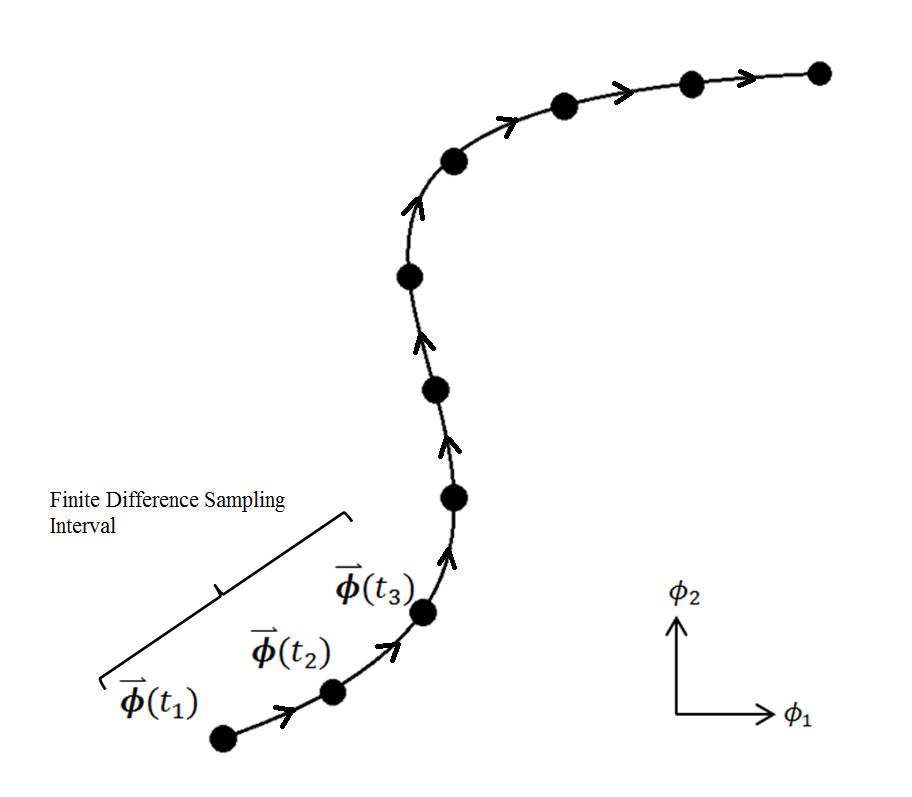
\includegraphics[scale=0.4]{rdagp.png}
\label{pathInFluxSpace}
\caption{A Path in 2D Flux space, where \textbf{totalPoints}=10 and \textbf{RDagSamplingPoints}=3}
\end{figure}
\newline
\newline
In conclusion, the user should first choose \textbf{totalPoints} such that the resolution of the system accurately captures the evolution of the eigensystem of $H_0(\phi(t))$ along the flux path. They should then choose an \textbf{RdagSamplingPoints} such that the error in the finite difference formula is minimized for the point spacing established by \textbf{totalPoints.}
\subsection{dHdphiSamplingPoints and dHdphiFiniteDifferenceSize}
To evaluate the coefficients of the taylor series expansion of a Hamiltonian in the instantaneous eigenbasis, $H(\phi(t))$, we must differentiate in flux space around the ideal flux path:
\begin{equation}
C_t(n,\vec{r}) = \frac{\partial^n H(\vec{\phi}(t)+ \vec{\xi}(t))} {\partial \xi_{r_1}\partial \xi_{r_2}...\partial \xi_{r_n}}  |_{\vec{\xi}=\vec{0}}
\end{equation}
If the user chooses $\mbox{\textbf{taylorExpansionOrder}} = 1$, the program will build $H(\vec{\phi}(t)+\vec{\xi}(t))$ at discrete intervals along each direction in flux space, and apply a central finite difference formula. If the user chooses $\mbox{\textbf{taylorExpansionOrder}} \geq 2$, the $C_t(n,\vec{r})$ matrices will contain mixed partial derivatives and the program will build $H(\vec{\phi}(t)+\vec{\xi}(t))$ along a hyper-dimensional mesh. See Fig.~(\ref{DiffBetTO1amdTOHigh}).
\newline
\newline
\begin{figure}
\centering
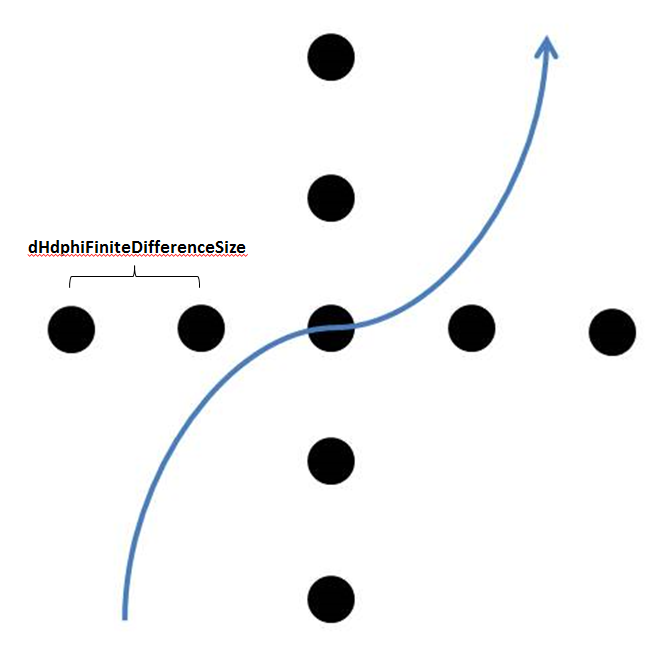
\includegraphics[scale=0.45]{TELow.png} 
\quad \quad \quad \quad
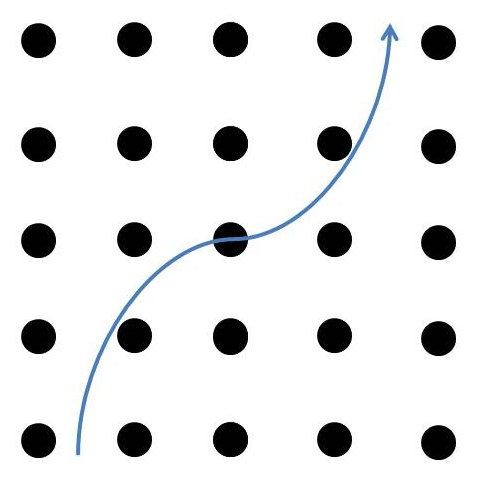
\includegraphics[scale=0.6]{TEHigh.png}
\label{DiffBetTO1amdTOHigh}
\caption{An illustration of the finite difference mesh in 2-dimensional flux space for evaluating the partial derivatives in $C_t(n,\vec{r})$. $H_0(\phi(t))$ is diagonalized at each one of these points. This mesh must be rebuilt at each stop along the ideal flux path. Here, \textbf{dHdphiSamplingPoints}$=5$. \newline Left: \textbf{taylorExpansionOrder} $= 1$. Right: \textbf{taylorExpansionOrder $\geq 2$}}
\end{figure}
The user must choose an odd number for the grid size, \textbf{dHdphiSamplingPoints} and a Real number for the spacing between grid points \textbf{dHdphiFiniteDifferenceSize}.
\newline
\newline
The user should pick these parameters such that error is minimized in the numerical derivatives, i.e. pick a point spacing that accurately captures the changes in the Hamiltonian, and then choose a number of sampling points that suits that point spacing. Note that increasing \textbf{dHdphiSamplingPoints} will increase the computational workload of the program. 
\section{Some Final Notes}
\subsection{Communication between successive diagonalization of $H_0(\phi(t))$}
A particularly tedious challenge in writing this code was building efficient communication between successive diagonalizations of $H_0(\phi(t))$. Crossing-eigenvalue degeneracies along a flux path are predicted with extrapolation, and then corrected. In addition, crossing-eigenvalue degeneracies are checked along the \textit{initial} interval used to calculate the partial derivatives in the coefficient matrices, $C_t(n,\vec{r})$. The correct ordering of the lowest eigenvalues is maintained over the time interval.
\newline
\newline
Discrete jumps in the global phases of the eigenvectors are also corrected. I.e, for any matrix $A$ and eigenvalue $\lambda$,
\begin{equation}
\begin{split}
\mbox{If } A \ket{\psi} = \lambda \ket{\psi} \\
\mbox{then } A (e^{i \phi} \ket{\psi}) = \lambda (e^{i \phi} \ket{\psi})
\end{split}
\end{equation}
for any real $\phi$. Large discontinuities in the global phases between successive sets of eigenvectors will result in an incorrect derivative in the non-adiabatic operator, $ \frac{d R^\dagger(\vec{\phi}(t))}{d t} $ in the off-diagonal entries. Large discontinuities are avoided by adjusting the global phase of each eigenvector such that the first entry of each eigenvector is a positive, real number. For a complex Hamiltonian, this will cause an overall "drift" in the phases of the eigenbasis, and therefore in the phases of the off-diagonal elements of the expansion coefficients. This something to keep in mind if you want to compare the output of this code to an analytic example (see the notebook \textit{Coefficient Test.nb} for such a comparison).
 We can convert between the initial ($\ket{\psi(t)}$) and instantaneous ($\ket{\psi(t)}'$) eigenbasis via the transformation
\begin{equation}
\ket{\psi(t)}' = R(\phi(t)) \ket{\psi(t)} \quad \quad \ket{\psi(t)} = R^\dagger (\phi(t)) \ket{\psi(t)}'
\end{equation}
\subsection{Interfacing with \textit{Mathematica}}
As it stands, the code is about as fast as it's going to be without significant overhaul. Fortunately, WSTP is a well-suited to inter-program communication, and all data exchanged between the C++ binary and \textit{Mathematica} notebook is highly efficient. Because Eigen3 has no Arnoldi partial diagonalization routine, diagonalizing $H_0({\phi(t)})$ in \textit{Mathematica} is the best way to do this right now anyway. I tried porting more of my code to lessen the communication load for WSTP, and possibly work exclusively in \textit{Mathematica}, but this actually lead to significant slowdown. In particular, large matrix addition in Eigen3 is fast enough to warrant keeping most of my program as a C++ binary. 
\newline
\newline
Further, I think usability is good as the program stands now. Dr. Kerman is able to write his Hamiltonians in \textit{Mathematica} as he prefers to do, and at least enjoy some scalability allowed by the low-level control of C++.
\subsection{Acknowledgments}
I want to thank Group 89 for giving me the opportunity to work at Lincoln Lab this summer, and I especially want to thank Dr. Obenland and Dr. Kerman for putting up with an intern; I know you guys are busy working on other things. I hope this code is useful to you guys, if you want me to run any simulations, or perform any maintenance on this, or add any additional features, please do not hesitate to contact me. 
\newline
\newline
Thanks again,\newline
--Jake
\begin{thebibliography}{9}
\bibitem{Fornberg} 
Fornberg, Bengt (1988), "Generation of Finite Difference Formulas on Arbitrarily Spaced Grids", Mathematics of Computation 51 (184): 699–706


\end{thebibliography}


\end{document}
